% compile with XeLaTeX
% this template was created by salim bou 
\documentclass[dvipsnames,mathserif,12pt]{beamer}
\mode<presentation>
\usepackage{xcolor}
\usepackage{mathtools}
\usepackage[LAE,T1]{fontenc}
\usepackage{hyperref}
 \RequirePackage{tikz}
\usetikzlibrary{calc}
\usetikzlibrary{shadows}
\usetikzlibrary{arrows,shapes}
\graphicspath{{figs/}}
\usepackage{polyglossia}
\setdefaultlanguage[numerals=maghrib,locale=algeria]{arabic} % locale=mashriq, libya, algeria, tunisia, morocco, or mauritania  for names of months in \date 
\setotherlanguage{english}
\newfontfamily\arabicfont[Script=Arabic]{Amiri}
\newfontfamily\arabicfontsf[Script=Arabic]{Amiri}

%\usetheme{Madrid}
\usetheme{modprogressbarMAHER}
%\usecolortheme{crane}
 
% for RTL liste
\makeatletter
\newcommand{\RTListe}{\raggedleft\rightskip\leftm}
\newcommand{\leftm}{\@totalleftmargin}
\makeatother

% RTL frame title
\setbeamertemplate{frametitle}
{\vspace*{-1mm}
  \nointerlineskip
    \begin{beamercolorbox}[sep=0.3cm,ht=2.2em,wd=\paperwidth]{frametitle}
        \vbox{}\vskip-2ex%
        \strut\hskip1ex\insertframetitle\strut
        \vskip-0.8ex%
    \end{beamercolorbox}
}

% align subsection in toc
\makeatletter
\setbeamertemplate{subsection in toc}
{\leavevmode\rightskip=5ex%
  \llap{\raise0.1ex\beamer@usesphere{subsection number projected}{bigsphere}\kern1ex}%
  \inserttocsubsection\par%
}
\makeatother

% RTL triangle for itemize
\setbeamertemplate{itemize item}{\scriptsize\raise1.25pt\hbox{\donotcoloroutermaths$\blacktriangleleft$}} 

%\setbeamertemplate{itemize item}{\rule{4pt}{4pt}}

\defbeamertemplate{enumerate item}{}
{\LR{
    %
    \hbox{%
    \usebeamerfont*{item projected}%
    \usebeamercolor[bg]{item projected}%
    \vrule width2.25ex height1.85ex depth.4ex%
    \hskip-2.25ex%
    \hbox to2.25ex{%
      \hfil%
      {\color{fg}\insertenumlabel}%
      \hfil}%
  }%
}}

\setbeamertemplate{enumerate item}[]

\setbeamertemplate{navigation symbols}{}
%%%%%%%%%%%%%%%%%%%%%%%%%%%%%%%%%%%%%%%%%%%%%%%%%%%%%%%%%%%%%%%%%%%%%%%%
% Reset the Itemize icon dimension and shape
%%%%%%%%%%%%%%%%%%%%%%%%%%%%%%%%%%%%%%%%%%%%%%%%%%%%%%%%%%%%%%%%%%%%%%%%
\setbeamertemplate{itemize item}{%
	\begin{tikzpicture}
	\shade[ball color=pbblue!95!white, preaction={fill=black,
		opacity=.25,transform canvas={xshift=1mm,yshift=-1mm, yscale=0.5}}] (0,0) circle (1.2ex);
	\end{tikzpicture}
}

\setbeamertemplate{itemize subitem}{%
	\begin{tikzpicture}
	\shade[ball color=pbgray!95!white, preaction={fill=black,
		opacity=.25,transform canvas={xshift=1mm,yshift=-1mm, yscale=0.5}}] (0,0) circle (1.0ex);
	\end{tikzpicture}
}
%%%%%%%%%%%%%%%%%%%%%%%%%%%%%%%%%%%%%%%%%%%%%%%%%%
\newenvironment{mycode}
    {%\RTListe
    \begin{center}
    \begin{tabular}{|p{0.9\textwidth}|}
    \hline\\
    }
    {
    \\\\\hline
    \end{tabular} 
    \end{center}
    }
%%%%%%%%%%%%%%%%%%%%%%%%%%%%[ blocks ]%%%%%%%%%%%%%%%%%%%%%%%%%%%%%%%%%%%%
\newenvironment<>{problock}[1]{%
	%\begin{actionenv}#2%
		\def\insertblocktitle{#1}%
		\par%
		\mode<presentation>{%
			%\setbeamercolor{block title}{fg=white,bg=blue!48!black}
			%\setbeamercolor{block body}{fg=white,bg=blue}
			  \setbeamercolor{itemize item}{fg=orange!20!black}
			%  \setbeamertemplate{itemize item}[triangle]
		}%
		\usebeamertemplate{block begin}}
	{\par\usebeamertemplate{block end}}%\end{actionenv}}
 %-------------------------------------------------------------------------
 \title{كورس مكثف لتعلم الLaTeX على محرر Overleaf}
\logo{
\includegraphics[width=0.5cm]{sudan_logo.png}}
\author[محمد ماهر]{ \href{https://www.facebook.com/mohammedmaher8932/}{\it{محمد ماهر عبد الرحيم محمد}}  }
\institute{\href{https://www.facebook.com/groups/651884204836245}{\Large{ملتقى الفيزيائيين السودانيين}} 
 
}
\vspace{-2cm}

\date{19/02/2023}
%--------------------------------------------------------------------------
%=========================================================================
\begin{document}

\begin{frame}

\begin{center}
\maketitle

\includegraphics[scale=0.1]{sfp.jpg}
    
\includegraphics[scale=0.2]{online-editor-2.png}
    
\includegraphics[scale=0.1]{sfp.jpg}
    
\end{center}

\end{frame}
%==========================================================
%///////////////////////////////////////////////////////////////////////////////////
\begin{frame}[plain]
	\addtocounter{framenumber}{-1}
	\begin{problock}{}
		\LARGE
		\vfill
		\centerline{\bf \textcolor{white}{\bf اليوم الثالث: أفضل الممارسات والتطبيقات
}}		
		\vfill
	\end{problock}
 
\end{frame}
%///////////////////////////////////////////////////////////////////////////////////
%==========================================================
\AtBeginSection[] {
\begin{frame}
\frametitle{المحتويات}
\tableofcontents[currentsection]
\end{frame}}
%\begin{frame}{المحتويات}
   % \tableofcontents
%\end{frame}
%==========================================================
\section{ إنشاء الأوامر الجديدة و تعريف البيئات الخاصة على ال \LaTeX}
\begin{frame}{ إنشاء الأوامر الجديدة على ال \LaTeX}
\scriptsize
\begin{center}
    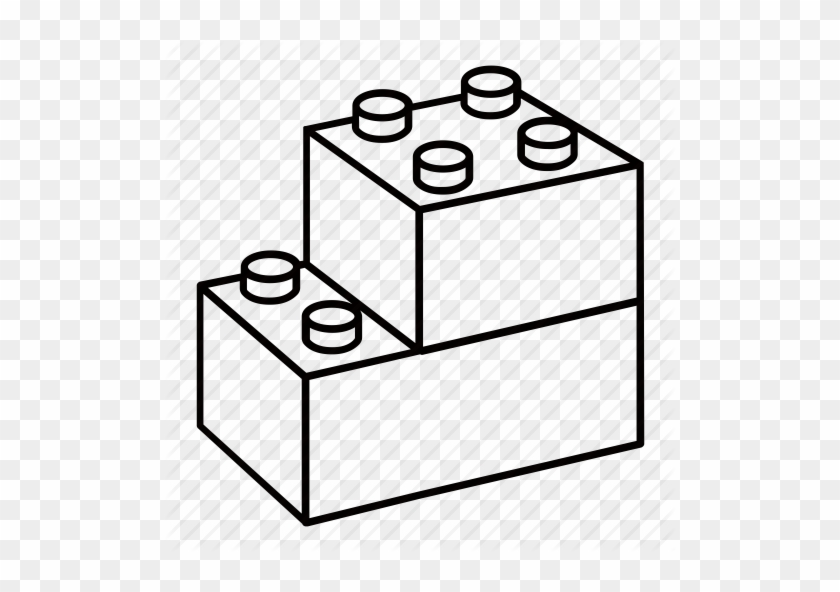
\includegraphics[scale=0.08]{lego.png}
\end{center}
غالبًا ما يصبح ضروريًا تعريف أوامرك الخاصة لتبسيط عملك أو تقليل المهام المتكررة أو إجراء بعض التنسيقات المعقدة.
 \begin{center}
   % \{مضمون الأمر\} [عدد المتغيرات] \{ اسم الأمر\} \sncommand{newcommand}
   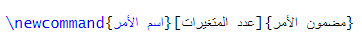
\includegraphics[scale=1]{newcommand.png}
 \end{center}
 \begin{itemize}\RTListe
     \item اسم الأمر: لابد ان يبدأ الاسم بوضع $\backslash$ قبل اختيار الاسم و بدون فراغ. 
     \item عدد المتغيرات: عدد المدخلات التى يجري عليها الأمر. 
     \item مضمون الأمر: الغرض المراد من الأمر القيام به.
     \item يتم الاشارة الى مكان المتغير بناءا على ترتيبه: المتغير( \#1 ) هو المكتوب في القوس الأول و (\#2 )  في الثاني و هكذا
 \end{itemize}

\end{frame}
%=========================================================
\subsection{التعامل مع المتغيرات}
\begin{frame}{حالة عدم وجود متغيرات}
 
\includegraphics[scale=1]{novar.png}
 \hrule\textline
    \begin{center}
        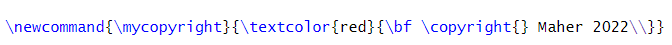
\includegraphics[scale=0.8]{example1.png}\\
        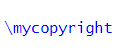
\includegraphics[scale=1]{useex1.png}\\
         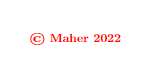
\includegraphics[scale=1]{outex1.png}
    \end{center}
\end{frame}
%=========================================================
\begin{frame}{حالة وجود متغير و أكثر}
\begin{columns}
\scriptsize
\column{0.6\textwidth}
\begin{mycode}
     \begin{center}
     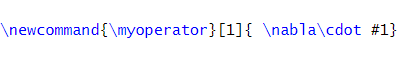
\includegraphics[scale=0.6]{onevar.png}\\
     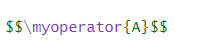
\includegraphics[scale=0.6]{onevars.png}
     $$\nabla\cdot A$$
 \end{center}
\end{mycode}
\column{0.5\textwidth}
\begin{mycode}
 \begin{center}
     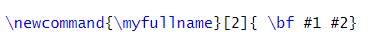
\includegraphics[scale=0.6]{twovar.png}\\
     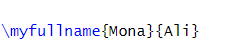
\includegraphics[scale=0.6]{towvars.png}\\
     \textbf{Ali Mona}
 \end{center}
 \end{mycode}
\end{columns}
\begin{center}
    \underline{\large إعادة تعريف أمر موجود مسبقا}\\
     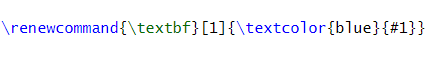
\includegraphics[scale=0.8]{renewcommmand.png}\\
     \vspace{-0.2cm}
      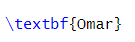
\includegraphics[scale=0.6]{renewcommmands.png}\\
      \vspace{-0.2cm}
      \textcolor{blue}{Omer}
\end{center}
\end{frame}
%============================================================
\subsection{البيئات الجديدة}
\begin{frame}{إنشاء بيئة جديدة}
\scriptsize
  \begin{center}
   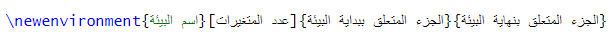
\includegraphics[scale=0.8]{newenvironment.png}
 \end{center}
 \begin{itemize}\RTListe
     \item  اسم البيئة: اي اسم تختاره و بدون وضع علامة ال$\backslash$.
     \item عدد المتغيرات: عدد المدخلات التى يجري مضمون البيئة من البداية للنهاية. 
     \item الجزء المتعلق ببداية البئية :تعريف الاجزاء البدائية للمحتوى.
     \item الجزء المتعلق بنهاية البئية :تعريف الاجزاء النهائية للمحتوى.
     \item يتم الاشارة الى مكان المتغير بناءا على ترتيبه: المتغير( \#1 ) هو المكتوب في القوس الأول و (\#2 )  في الثاني و هكذا
 \end{itemize}
\end{frame}
%==========================================================
\begin{frame}
\begin{flushleft}
 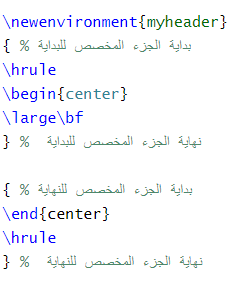
\includegraphics[scale=0.8]{newenvs2.png}
\end{flushleft}

\begin{center}
      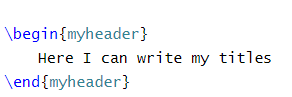
\includegraphics[scale=0.8]{sam.png}\\
       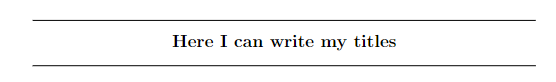
\includegraphics[scale=0.8]{newenvo.png}
\end{center}
    
\end{frame}
%==========================================================
\section{العروض التقديمة بإستخدام ال \LaTeX{} Beamer}
\begin{frame}{Beamer}
\scriptsize
 \begin{center}
     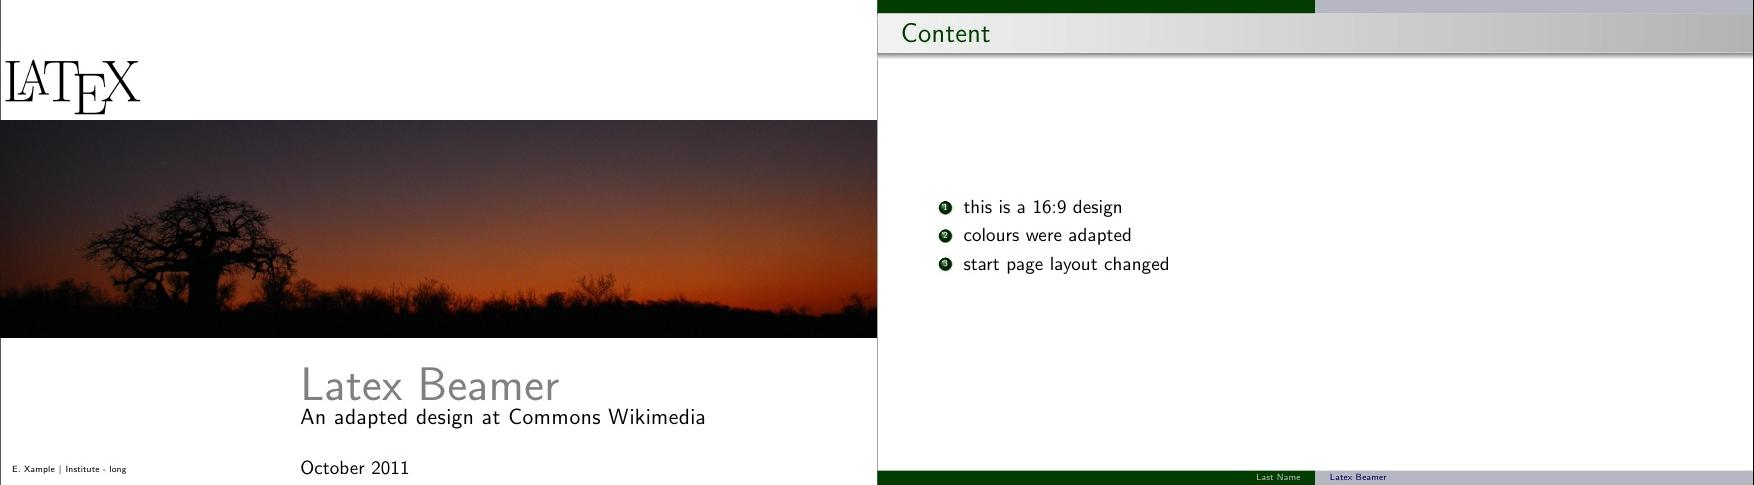
\includegraphics[scale=0.2]{A_modified_Latex_Beamer_example.jpg}
 \end{center}
 \underline{\bf المميزات}
 \begin{itemize}\RTListe
    \item يعمل على جميع مترجمات ال\LaTeX{}
    \item يمكن إنشاء التراكبات والتأثيرات الديناميكية بسهولة.
    \item يمكن تعديل مظهر العروض التقديمية باستخدام الأنساق "ثيمات".
    \item لا تزال الأوامر القياسية لل\LaTeX{} تعمل بنفس الكفاءة
    \item يمكن بسهولة تغيير التخطيط والألوان والخطوط المستخدمة في العرض التقديمي بشكل عام ، مع الحفاظ على التحكم في أدق التفاصيل.
    \item  الناتج النهائي عبارة عن ملف PDF ، مما يعني أن العرض التقديمي المحدد سيبدو دائمًا كما هو بغض النظر عن الجهاز الذي تم فتحه عليه.
 \end{itemize}
 
\end{frame}
%=========================================================
\begin{frame}{ابسط بداية}
\vspace{-0.5cm}
    \begin{center}
        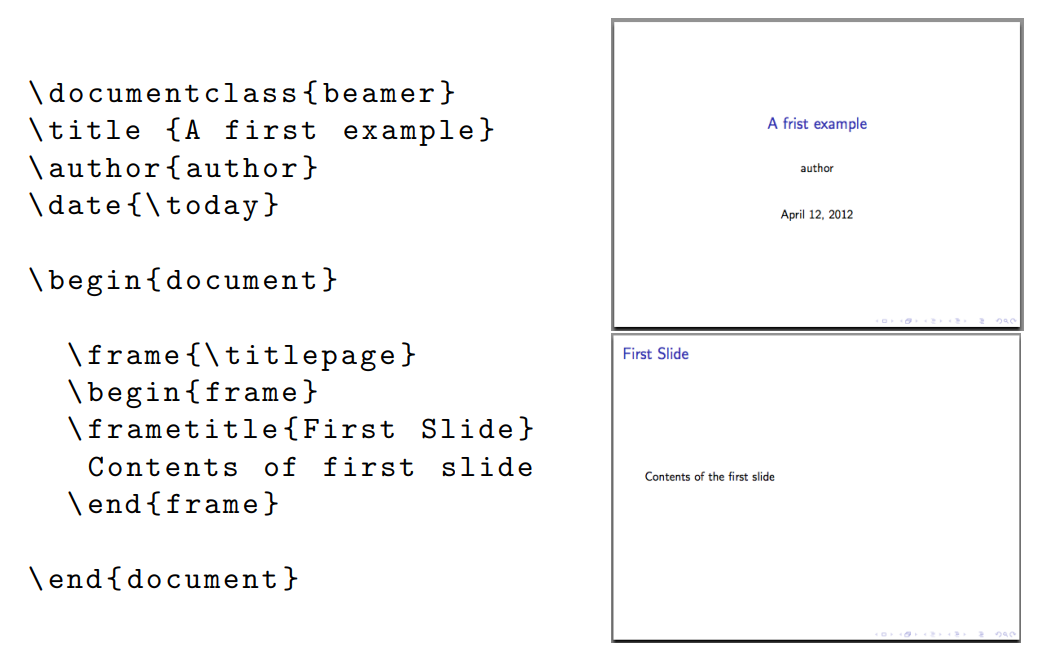
\includegraphics[scale=0.5]{fst.png}
    \end{center}
\end{frame}
%=========================================================
\subsection{الأقسام و قائمة المحتويات}
\begin{frame}{استخدام الاقسام}
    \begin{itemize}
        \item تعامل مع الأقسام كما تعلمنا في السابق  .
        \item
استخدم tableofcontents$\backslash$ لإبقاء الجمهور على اطلاع بالخطة العامة للعرض.
\item استخدم ال AtBeginSection$\backslash$ لمساعدة الجمهور
اتبع هيكل حديثك.
    \end{itemize}
\begin{center}
    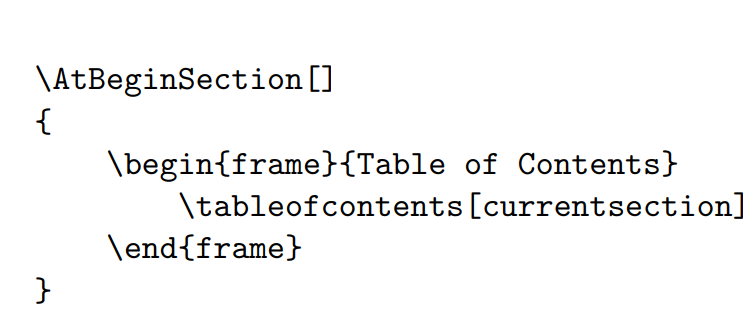
\includegraphics[scale=0.6]{secs.png}
\end{center}
\end{frame}
%=========================================================
\subsection{محتوى الاطارات او القوالب}
\begin{frame}{الأعمدة و التحكم في ابعاد الاطار}
لتنسيق هيكل اي إطار يمكن استخدام الاعمدة كالتالي:
\begin{center}
     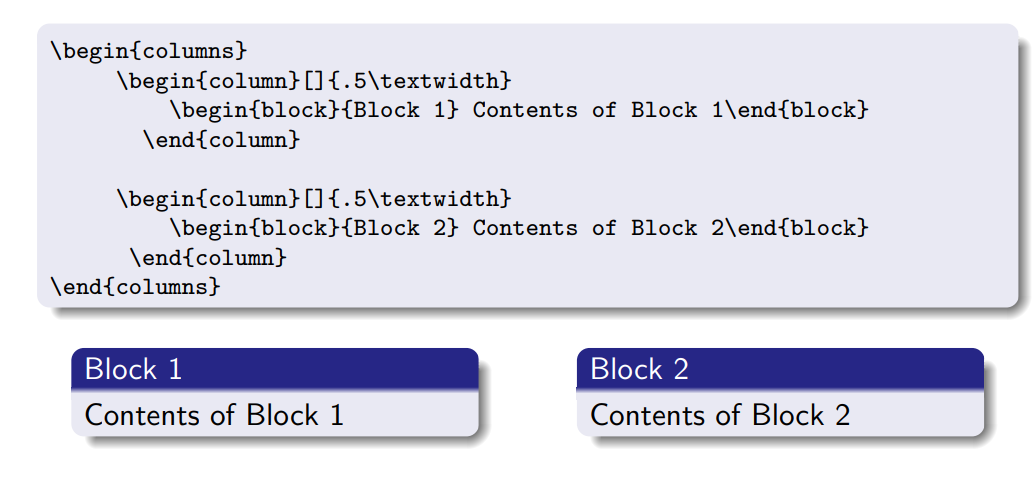
\includegraphics[scale=0.5]{ols.png}
 \end{center}
\end{frame}
%=========================================================
\subsection{المظهر الكلي لملف العرض}
\scriptsize
\begin{frame}{الانساق او ما يعرف بالثيمات}
بالنسبة إلى مظهر العرض التقديمي ، يمكنك تحديد ثيمات محددة مسبقًا
من فئة Beamer. وبالتالي ، يصنف Beamer خمس فئات:
\begin{itemize}
    \item  ثيمات العرض التقديمي: قالب الشرائح
\item نسق ألوان : مخطط ألوان لقالب الشريحة
\item ثيمات الخطوط : يحدد الخطوط
\item ثيمات داخلية : تحدد داخل الشريحة مثل الرصاص والصناديق وما إلى ذلك.
\item ثيمات خارجية : تحدد خارج الشريحة مثل خطوط الرأس والقدم
\end{itemize}
\begin{center}
    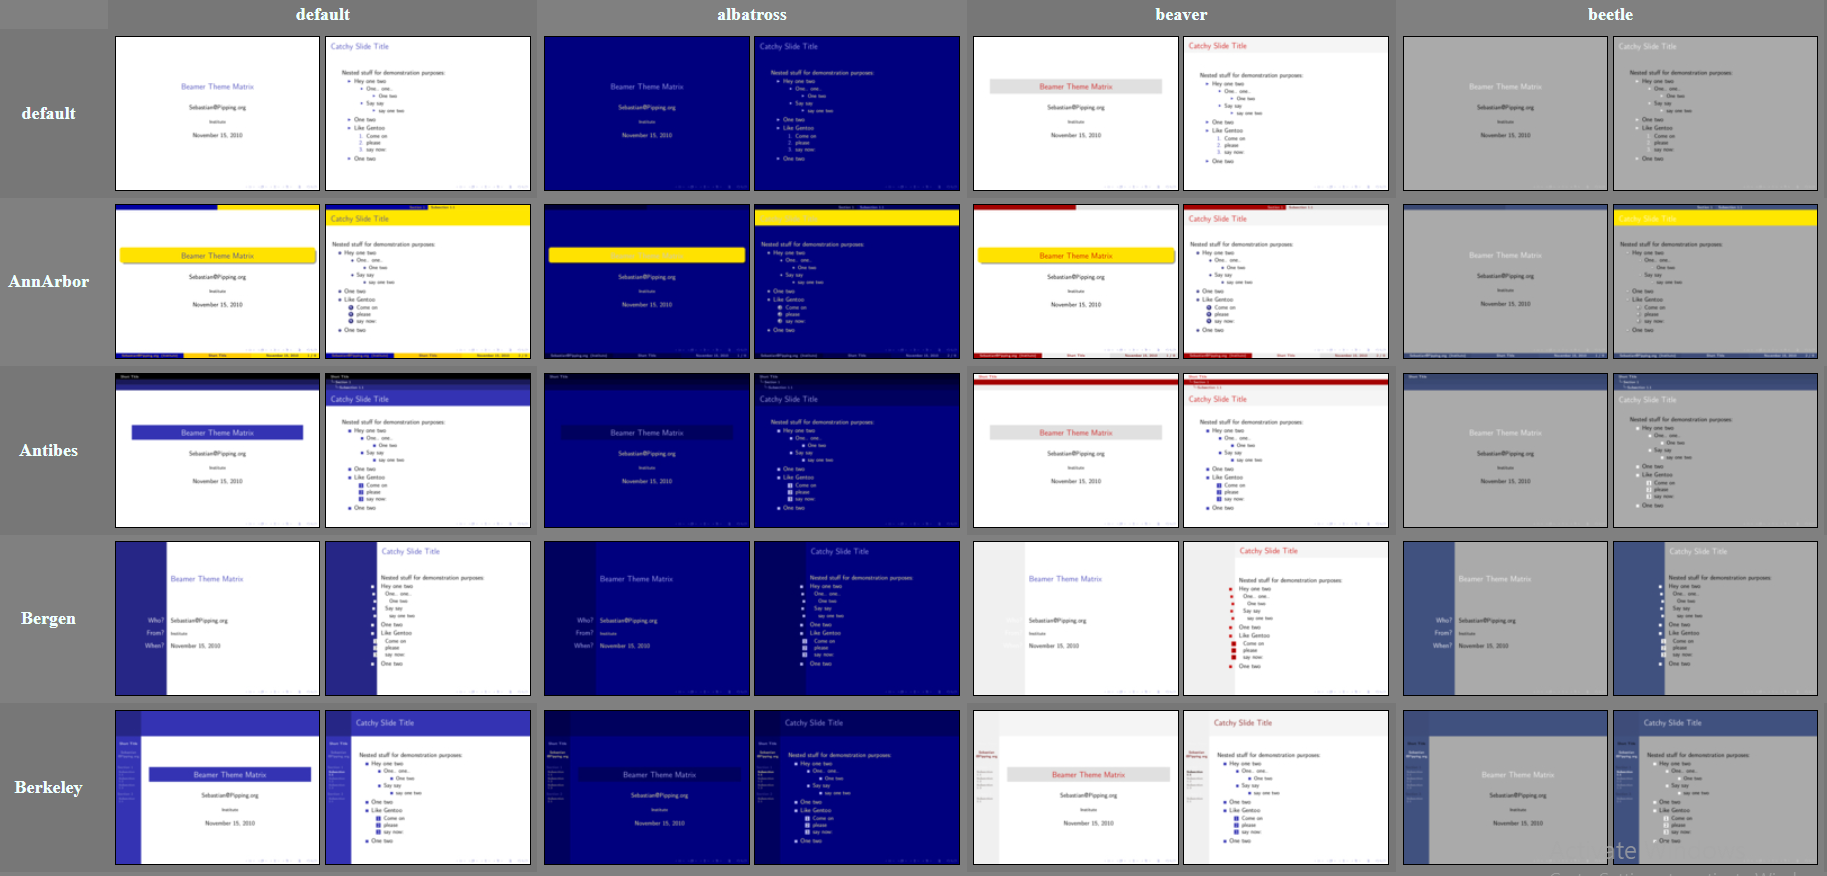
\includegraphics[scale=0.2]{matrix.png}
\end{center}
\end{frame} 
%=========================================================
\begin{frame}{الثيمات المعتمدة}
\begin{itemize}
    \item     من اجل اداج الثيمة المختارة استخدم الامر: \{اسم الثيمة \} usetheme$\backslash$
\itemمن اجل اختيار اللون المتاح مع كل ثيمة استخدم:د usecolortheme$\backslash$
\end{itemize}
       \begin{center}
    \begin{itemize}\RTListe
        \item الثيمات المعتمدة:
    \end{itemize}
        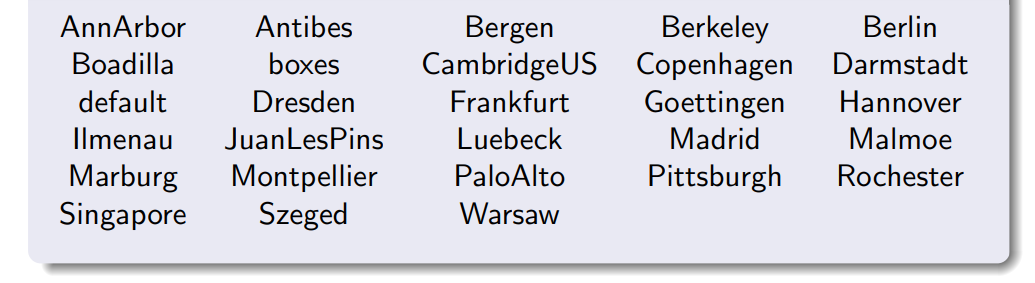
\includegraphics[scale=0.5]{themes.png}\\
        \begin{itemize}\RTListe
        \item  الوانها المتوفرة:
    \end{itemize}
        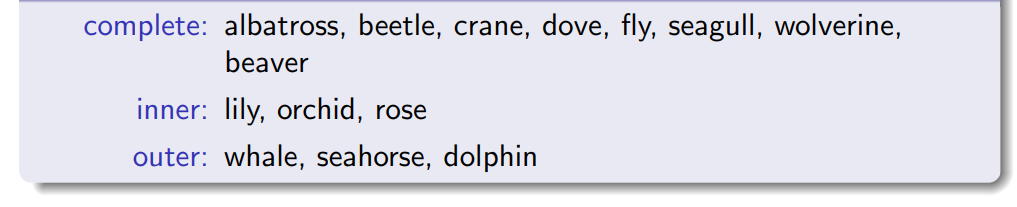
\includegraphics[scale=0.5]{cololstherms.png}\\
        \href{https://hartwork.org/beamer-theme-matrix/}{https://hartwork.org/beamer-theme-matrix/}
    \end{center}

\end{frame}

\begin{frame}{خاتمة}

\includegraphics[scale=0.2]{expert.png}
    \begin{itemize}
        \item تعلم مهارات متقدمة في اللاتك عملية مستمرة
        \item احسن وسيلة للتعلم هو ان يكون لكن عمل ترغب في انجازه
        \item تذكر ان الحيرة و التشويش اول خطوة في طريق الفهم
        \item و ارتكاب الأخطاء هو خطواة الثانية مباشرة في طريقك نحو التعلم العميق
    \end{itemize}
\end{frame}
\end{document}
